\documentclass{beamer}
\usepackage[utf8]{inputenc}
\usepackage[T2A]{fontenc}
\usepackage[english, russian]{babel}
%\usepackage[sfdefault, light]{roboto}
\usepackage{epstopdf}
\usepackage[font={footnotesize}, labelfont={footnotesize}]{caption}
\usepackage[font={footnotesize}, labelfont={footnotesize}]{subcaption}
\usepackage{bm}
\usepackage{algpseudocode}
\usepackage[absolute,overlay]{textpos}
  \setlength{\TPHorizModule}{1mm}
  \setlength{\TPVertModule}{1mm}

\usepackage{tikz}

% Operators
\DeclareMathOperator{\argmax}{argmax}
\DeclareMathOperator{\argmin}{argmin}

% Listings
\usepackage{listings}
\definecolor{codegreen}{rgb}{0,0.6,0}
\definecolor{codegray}{rgb}{0.5,0.5,0.5}
\definecolor{codepurple}{rgb}{0.58,0,0.82}
\definecolor{backcolour}{rgb}{0.95,0.95,0.92}
 
\lstdefinestyle{pythonstyle}{
    backgroundcolor=\color{backcolour},   
    commentstyle=\color{codegreen},
    keywordstyle=\color{magenta},
    numberstyle=\tiny\color{codegray},
    stringstyle=\color{codepurple},
    basicstyle=\scriptsize,
    breakatwhitespace=false,         
    breaklines=true,                 
    captionpos=b,                    
    keepspaces=true,                 
    numbers=left,                    
    numbersep=5pt,                  
    showspaces=false,                
    showstringspaces=false,
    showtabs=false,                  
    tabsize=2
}
\lstset{style=pythonstyle, language=Python}

\graphicspath{ {images/} }
\setbeamertemplate{caption}{\raggedright\insertcaption\par}
\def\figurename{}

\title{Методы оптимизации для задач на графах}
\date[\today]{Практика по дисциплине <<Основы алгоритмов>>\\\today}
\author[Anton]{Першин Антон Юрьевич, Ph.D.}

\institute{Программа <<Большие данные и распределенная цифровая платформа>>\\Санкт-Петербургский государственный университет}

\usetheme{tonythequick}


\begin{document}

\begin{frame}
\titlepage
\end{frame}

\setcounter{framenumber}{0}

\section{}

\begin{frame}{Линейное программирование}
    \small

    \begin{definition}
        Линейной программой называется задача оптимизация с линейной целевой функцией и линейными ограничениями (равенствами и неравенствами):
        \begin{align*}
            \argmax_{\bm{x}} &\bm{c}^T \bm{x} \\
            \text{s.t.} &\bm{A}_{eq} \bm{x} = \bm{b}_{eq} \\
            &\bm{A}_{ub} \bm{x} \leq \bm{b}_{ub} \\
            &\bm{A}_{lb} \bm{x} \geq \bm{b}_{lb}
        \end{align*}
    \end{definition}

    \begin{minipage}{0.49\textwidth}
        {\bf \centering Стандартная форма}
        \begin{align*}
            \argmax_{\bm{x}} &\bm{c}^T \bm{x} \\
            \text{s.t.} &\bm{A} \bm{x} \leq \bm{b} \\
            &\bm{x} \geq \bm{0}
        \end{align*}
        \vfill
    \end{minipage}
    \begin{minipage}{0.49\textwidth}
        {\bf \centering Каноническая форма}
        \begin{align*}
            \argmax_{\bm{x}} &\bm{c}^T \bm{x} \\
            \text{s.t.} &\bm{A} \bm{x} = \bm{b} \\
            &\bm{x} \geq \bm{0}
        \end{align*}
        \vfill
    \end{minipage}
\end{frame}

\begin{frame}{Кратчайший путь как линейная программа}
    \small

    Введем обозначения:
    \begin{itemize}
        \item $w(u, v)$ -- вес ненаправленного или направленного ребра $u \to v$;
        \item $s$ -- начальный узел пути;
        \item $t$ -- конечный узел пути;
        \item $x(u, v)$ -- бинарная переменная, указывающая, включено ли ребро $u \to v$ в путь.
    \end{itemize}

    Линейная программа поиска кратчайшего пути на графе:
    \begin{align*}
        \argmin_{\bm{x}} &\sum_{(u, v) \in E} w(u, v) x(u, v) \\
        \text{s.t.} &\sum_{u \in V} x(u, t) - \sum_{w \in V} x(t, w) = 1 \\
        &\sum_{u \in V} x(u, v) - \sum_{w \in V} x(v, w) = 0 \quad \forall v \in V \backslash \{s, t\} \\
    \end{align*}
\end{frame}

\begin{frame}{Поиск восхождением к вершине (Hill Climbing)}
    \small

    Hill Climbing -- стохастический итерационный алгоритм локального поиска.

    
\begin{algorithmic}[1]
\State $n \gets $ number of tweak desired to sample the gradient
\State $S \gets $ some initial candidate solution
\Repeat
    \State $R \gets \text{Tweak}(\text{Copy}(S))$
    \For{$n-1$ times}
        \State $W \gets \text{Tweak}(\text{Copy}(S))$
        \If{\text{Quality}(W) > \text{Quality}(R)}
            \State $R \gets W$
        \EndIf
    \EndFor
    \If{\text{Quality}(R) > \text{Quality}(S)}
        \State $S \gets R$
    \EndIf
\Until{$S$ is the ideal solution or we have run out of time}\\
\Return S
\end{algorithmic}
\end{frame}

\begin{frame}{Имитация отжига (Simulated Annealing)}
    \small

    Имитация отжига -- стохастический итерационный алгоритм глобального поиска.

    
\begin{algorithmic}[1]
\State $t \gets $ temperature
\State $S \gets $ some initial candidate solution
\State $\xi \gets $ random value generator yielding a random value from 0 to 1 each time it is accessed
\State $Best \gets S$
\Repeat
    \State $R \gets \text{Tweak}(\text{Copy}(S))$
    \If{\text{Quality}($R$) > \text{Quality}($S$) or $\xi < \exp[\frac{\text{Quality}(R) - \text{Quality}(S)}{t}]$}
        \State $S \gets R$
    \EndIf
    \State{Decrease $t$}
    \If{\text{Quality}($S$) > \text{Quality}($Best$)}
        \State $Best \gets S$
    \EndIf
\Until{$Best$ is the ideal solution or we have run out of time or $t \leq 0$}\\
\Return $Best$
\end{algorithmic}
\end{frame}

\begin{frame}{Раскраска графов}
    \small

    \begin{minipage}{0.49\textwidth}
        Раскраска графа предполагает присваивание одного из $k$ цветов каждой вершине таким образом, чтобы у любых двух смежных вершин были несовпадающие цвета.
    \end{minipage}
    \begin{minipage}{0.49\textwidth}
        \begin{figure}
            \centering
            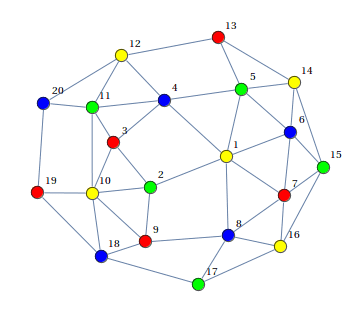
\includegraphics[width=1.0\textwidth]{images/graph_coloring.png}
            \caption{4-раскраска графа.}
        \end{figure}
    \end{minipage}

    Зачастую количество цветов меньше хроматического числа, что требует поиска решения, минимизирующего количество конфликтов, то есть количество ребер с узлами одинаковых цветов.
    Кроме того, раскраска графов в общем случае является NP-сложной задачей.
\end{frame}

\begin{frame}{Разбиение графов}
    \small

    \begin{minipage}{0.49\textwidth}
        Разбиение графа $G = (V, E)$ в $k$ компонент предполагает такое разбиение $V = \bigcap_i V_i$, что сумма весов ребер, разделяющих компоненты, минимальна.
    \end{minipage}
    \begin{minipage}{0.49\textwidth}
        \begin{figure}
            \centering
            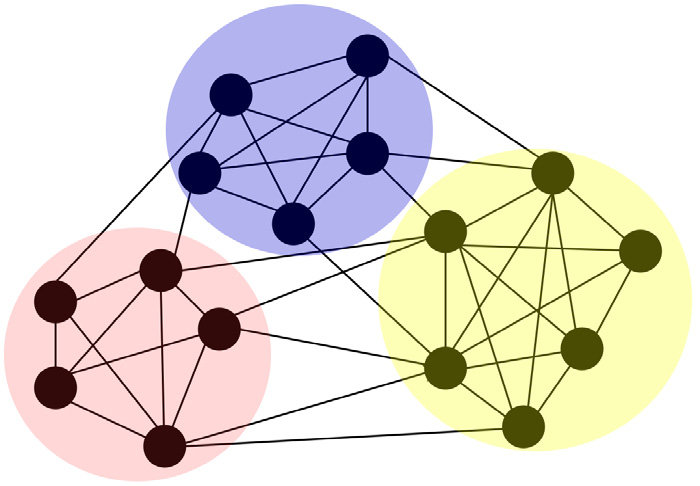
\includegraphics[width=1.0\textwidth]{images/graph_partitioning.png}
            \caption{Разбиение графа по 3 компонентам.}
        \end{figure}
    \end{minipage}

    Эта задача находится множество применений: проектирование топологий сетей, балансировка награзки в вычислительных системах, задачи теории расписаний и так далее.
    Разбиение графов в общем случае является NP-сложной задачей.
\end{frame}

\begin{frame}{Спектральная кластеризация}
    \small

    Одним из способов решения задачи разбиения графа является спектральная кластеризация:

    \begin{enumerate}
        \item Построить матрицу смежности $\bm{A}$
        \item Построить диагональную матрицу $\bm{D}$, где $D_{ii} = \sum_j A_{ij}$
        \item Найти лапласиан графа: $\bm{L} = \bm{D} - \bm{A}$
        \item Найти разложение $\bm{L}$ на собственные числа и собственные вектора
        \item Первый собственный вектор (предполагается сортировка от наименьшего собственного числа к наибольшему) содержит информацию о компонентах связности
        \item Остальные вектора по порядку можно использовать как признаки для кластеризации (например, с помощью k-means) 
    \end{enumerate}
\end{frame}

\end{document}
